\documentclass[letterpaper,12pt]{article}

\usepackage{ucs}
\usepackage[utf8x]{inputenc}
\usepackage{amsmath}
\usepackage{amsfonts}
\usepackage{amssymb}
\usepackage[margin=1in]{geometry}
\usepackage{enumerate}
\usepackage{graphicx}

\newcommand{\abs}[1]{\lvert #1\rvert}
\newcommand{\len}[1]{\lVert #1\rVert}
\newcommand{\R}{\mathbb{R}}
\newcommand{\x}{\mathbf{x}}
\newcommand{\y}{\mathbf{y}}
\newcommand{\inter}[1]{\overset{\,\,\circ}{#1}}
\newcommand{\T}{\mathcal{T}}
\newcommand{\N}{\mathbb{N}}
\DeclareMathOperator{\Int}{Int}

\title{Math 4310 Assignment \#5 Solutions\\University of Lethbridge, Fall 2014}
\author{Sean Fitzpatrick}
\begin{document}
 \maketitle

\begin{enumerate}
\item If $X\times Y$ has the product topology, and $A\subseteq X$, $B\subseteq Y$, show that $\overline{A\times B} = \overline{A}\times \overline{B}$, $(A\times B)^\circ = \inter{A}\times\inter{B}$, and $\partial (A\times B) = \partial A\times \partial B$.

\bigskip

\noindent {\bf Solution}: We first consider $\overline{A\times B}$. We know that $(x,y)\in \overline{A\times B}$ if and only if every neighbourhood of $(x,y)$ contains a point of $A\times B$. Since every open neighbourhood contains a basic open set (and can be written as a union of basic open sets), it follows that $(x,y)\in\overline{A\times B}$ if and only if for every set $U\times V\subseteq X\times Y$, where $U$ is open in $X$ and $V$ is open in $Y$, and $(x,y)\in U\times V$, we have $(U\times V)\cap (A\times B)\neq \emptyset$. But then we have that $(a,b)\in (U\times V)\cap (A\times B)$ if and only if $a\in U\cap A$ and $b\in V\cap B$, which is equivalent to having $x\in\overline{A}$ and $y\in\overline{B}$, or $(x,y)\in \overline{A}\times \overline{B}$.

Similarly, a point $(x,y)\in A\times B$ is an interior point if and only if there exists a basic open set $U\times V$ with $(x,y)\in U\times V\subseteq A\times B$, which is if and only if there exist open sets $U\subseteq X$ and $V\subseteq Y$ such that $x\in U\subseteq A$ and $y\in V\subseteq B$, and this is if and only if $(x,y)\in \inter{A}\times\inter{B}$.

Finally, we have that 
\[
\partial(A\times B) = \overline{A\times B}\setminus (A\times B)^\circ = (\overline{A}\times \overline{B})\setminus (\inter{A}\times \inter{B}) = (\overline{A}\setminus \inter{A})\times (\overline{B}\setminus \inter{B}) = \partial A\times \partial B.
\]



\item Given a countable number of spaces $X_1,X_2,\ldots$, the product $X=\prod_i X_i$ is the set of all points of the form $x=(x_1,x_2,\ldots)$, where $x_i\in X_i$ for $i=1,2,\ldots$. The product topology on $X$ is defined to be the coarsest topology for which all of the projections $\pi_i:X\to X_i$ are continuous. (This is sometimes known as the {\em weak} product topology.)
\begin{enumerate}
 \item Construct a basis for this topology in terms of the open subsets of the spaces $X_1,X_2,\ldots$.

\bigskip

\noindent {\bf Solution}: Since we want the product topology on $X$ to be the coarsest for which all of the projections $\pi_i:X\to X_i$ are continuous, we define the product topology to be the topology generated by the subbasis
\[
 \mathcal{S} = \{\pi_i^{-1}(U_i) : U_i\subseteq X_i \text{ is open }, i=1,2,3,\ldots\}.
\]
(We see that this is indeed a subbasis since for any $i\in\N$, $\pi_i^{-1}(X_i) = X\in \mathcal{S}$, so it's certainly the case that $X\subseteq \bigcup_{S\in\mathcal{S}}S$.) The open sets in the subbasis are thus of the form
\[
 \pi_i^{-1}(U_i) = X_1\times \cdots \times X_{i-1}\times U_i \times X_{i+1}\times\cdots.
\]
The resulting basis $\mathcal{B}$ is obtained from $\mathcal{S}$ by taking finite intersections; thus, a basic open set is of the form
\[
 B = \prod_{i=1}^\infty A_i,
\]
where for some finite subset $I=\{i_1,i_2,\ldots, i_k\}\subseteq \N$ we have $A_i = U_i$ for $i\in I$ and $U_i\subseteq X_i$ an open subset, and $A_j = X_j$ for all $j\notin I$. In other words, a basic open set is a product of sets $A_i\subseteq X_i$, where $A_i$ is a proper open subset of $X_i$ for at most finitely many $i\in\N$.

\item (In which a hint for part (a) is given.) The {\em box topology} on $X=\prod_i X_i$ is the topology defined by the basis $\mathcal{B} = \{U_1\times U_2\times \cdots \,|\, U_i \text{ is open in } X_i, i=1,2,\ldots\}$. Show that the box topology contains the product topology in part (a) (this is your hint: your answer for (a) should be different than the basis in (b)!), and that the two sets are equal if and only if $X_i$ has the indiscrete topology for all but finitely many values of $i$.
\end{enumerate}

\bigskip

\noindent {\bf Solution}: Since each $X_i$ is an open subset of itself, we can take $U_i=X_i$ for all but finitely many $i\in\N$, and this will be a basic open subset in the box topology. But such sets are precisely the basic open subsets of the product topology. Thus, the box topology contains the product topology, since the basis for the former contains the basis for the latter.

In order for the two topologies to coincide, we would need to guarantee that at most finitely many of the $U_i$ in a basic open set $U_1\times U_2\times\cdots$ of the box topology are proper open subsets of their respective spaces $X_i$. Since the box topology allows each $U_i$ to be any open subset, this is possible if and only if there are only finitely many $X_i$ for which there exists a nonempty proper subset $U_i\subseteq X_i$, and this is if and only if the remaining spaces are equipped with the indiscrete topology.
\end{enumerate}
For problems 3 and 4, the diagonal map $\Delta:X\to X\times X$ is given by $\Delta(x) = (x,x)$, and the {\em diagonal} in $X\times X$ is the image $\Delta(X) = \{(x,x)\,|, x\in X\}$ of the diagonal map.

\begin{enumerate}
\setcounter{enumi}{2}
\item Prove that a topological space $X$ is discrete if and only if $\Delta(X)$ is an open subset of $X\times X$ in the product topology.

\bigskip

\noindent {\bf Solution}: If the topology on $X$ is discrete, then $\{x\}\times\{y\}\subseteq X\times X$ is open for any $x,y\in X$. It follows that the topology on $X\times X$ is discrete, since any subset can be written as a union of its points. In particular, the diagonal $\Delta(X)$ must be open in $X\times X$.

Conversely, suppose that $\Delta(X)$ is open in $X\times X$. Then for any $(x,x)\in \Delta(X)$ there must exist open sets $U,V\subseteq X$ such that $x\in U$, $x\in V$, and $U\times V\subseteq \Delta(X)$. If $U\neq \{x\}$ then we can find some $y\in U$ with $y\neq x$, which implies that $(y,x)\in U\times V\subseteq \Delta(X)$, but this is impossible, since $\Delta(X)$ contains only points of the form $(x,x)$. Thus, we must have $U=\{x\}$, and since this is open in $X$, the topology on $X$ must be discrete.

\item Prove that $X$ is Hausdorff if and only if $\Delta(X)$ is a closed subset of $X\times X$ in the product topology.

\bigskip

\noindent {\bf Solution}: Suppose $X$ is Hausdorff, and let $(x,y)\in X\times X$ be any point with $x\neq y$. Then we can choose disjoint open sets $U,V\subseteq X$ with $x\in U$ and $Y\in V$. The $(x,y)\in U\times V$, and since $U$ and $V$ are disjoint, no point of the form $(x,x)$ can be contained in $U\times V$, so $U\times V\subseteq X\times X\setminus \Delta(X)$. It follows that $\Delta(X)$ is closed.

Conversely, suppose that $\Delta(X)$ is closed in $X\times X$. Then $X\times X\setminus \Delta(X)$ is open. Therefore, given any $x,y\in X$ with $x\neq y$, $(x,y)\in X\times X\setminus \Delta(X)$, so there exists a basic open set $U\times V$ with $(x,y)\in U\times V\subseteq X\times X\setminus \Delta(X)$. We claim that $U$ and $V$ must be disjoint. If not, there would exist some $z\in U\cap V$, and hence $(z,z)\in (U\times V)\cap \Delta(X)$. But this is impossible, since $U\times V$ is contained in the complement of $\Delta(X)$.

\item Suppose that $X$ is Hausdorff.
\begin{enumerate}
 \item Show that $\{x\}$ is closed, for any $x\in X$.

\bigskip

\noindent {\bf Solution}: We already proved in class that finite point sets are closed in a $T_1$ space, so one option is to prove that Hausdorff implies $T_1$: if $X$ is Hausdorff, given any $x\neq y$, we can choose {\em disjoint} open sets $U$ and $V$ containing $x$ and $y$, respectively, so it's certainly the case that $x\in U$ and $y\notin U$, while $y\in V$ and $x\notin V$, which shows that $X$ is $T_1$.

Alternatively, let $A=\{x\}$. Then $A$ is closed if and only if $A^c = X\setminus\{x\}$ is open. Choosing any $y$ in $A^c$, we must have $y\neq x$, since $x\notin A^c$, and thus there exists an open set $U$ with $y\in U$ and $x\notin U$, which implies that $U\subseteq A^c$.
Hence, $A^c$ is open and thus $A=\{x\}$ is closed.

 \item Let $\mathcal{U}$ denote the collection of all open neighbourhoods of some $x\in X$. Prove that $\bigcap_{U\in \mathcal{U}}U = \{x\}$.

\bigskip

\noindent {\bf Solution}: It's clear that $x\in\bigcap_{U\in\mathcal{U}}U$, since every $U\in\mathcal{U}$ contains $x$. Suppose that $y\neq x$. Since $X$ is Hausdorff, there exists $U\in\mathcal{U}$ with $y\notin U$, and thus, $y\notin \bigcap_{U\in\mathcal{U}}U$.
\end{enumerate}
 \item Suppose that $X$ is an infinite set with the finite complement (co-finite) topology.
\begin{enumerate}
 \item Show that $\{x\}$ is closed, for any $x\in X$.

\bigskip

\noindent {\bf Solution}: Since $X\setminus\{x\}$ is open (its complement is $\{x\}$, a finite set), $\{x\}$ is closed.

 \item Show that, in spite of part (a), $X$ is not Hausdorff.

\bigskip

For $X$ to be Hausdorff, given $x\neq y$ we would have to be able to find disjoint open sets $U$ and $V$ containing $x$ and $y$, respectively. But it is not even possible to find disjoint open sets: if $U$ is open, then $X\setminus U$ is finite. If $U\cap V=\emptyset$, we would have to have $V\subseteq X\setminus U$, which would imply that $V$ is finite, and thus $V$ cannot be open, since $X$ is infinite and thus so is $X\setminus V$.

 \item Let $\mathcal{U}$ denote the collection of all open neighbourhoods of some $x\in X$. Show that it is not true that $\bigcap_{U\in \mathcal{U}}U = \{x\}$.

\bigskip

\noindent {\bf Solution}: This, unfortunately, {\bf IS} true! I meant to ask a different question but clearly was in a hurry or half asleep. If you look at the proof for 5(b), you'll see that it only requires the $T_1$ axiom, and not the full strength of the Hausdorff axiom. Indeed, for any $y\neq x$, $X\setminus \{y\}$ is an open neighbourhood of $x$ that does not contain $y$, so $y\notin \bigcap U$.

The problem should have asked you to show both this and 6(a), and {\em then} note that in spite of both of these things being true, $X$ is not Hausdorff. Basically this is 11.6(b) from the text. So anyway, free points for everyone and I'll try to indicate where you went wrong in attempting to prove the impossible.

\end{enumerate}
{\bf Bonus problem}: Consider the following diagram, where we have the square $[0,1]\times [0,1]$ and the circle with centre $(1/2,1/2)$ and radius $\sqrt{2}/2$:
\begin{center}
 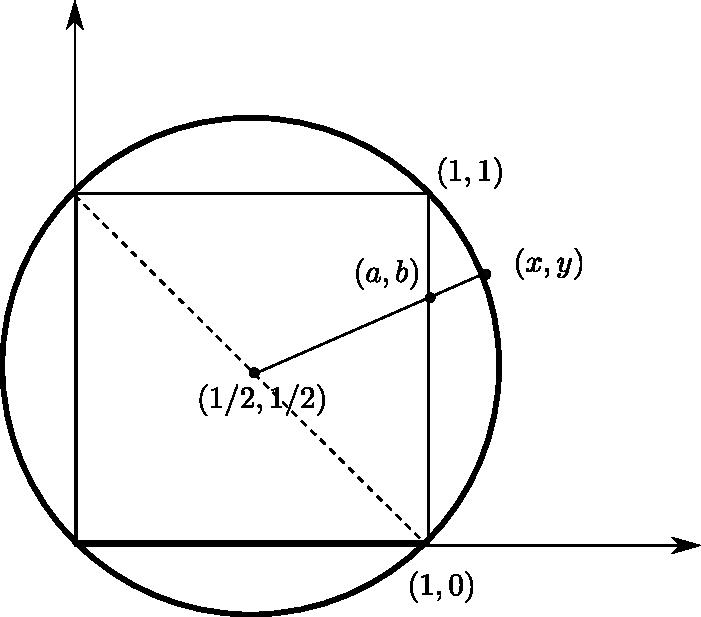
\includegraphics[width=3in]{Bonus.pdf}
\end{center}
We map the square onto the circle via ``radial expansion'': for the right-hand side of the square note that the points $(a,b)$ and $(x,y)$ lie on the same line, and that $a=1$. If we let $\theta$ denote the angle between this line and the line $y=1/2$, we have $b=\tan\theta$, and thus $y=x\tan\theta = xb$. Using the equation of the circle (I'm leaving out the details) we can write the point $(x,y)$ on the circle in terms of $b\in [0,1]$.

Now, if $(a,b)$ is any point inside the square; in particular, inside the triangle bounded by $x=y$, $y=1-x$, and $x=1$, we can apply the same procedure, and map $(a,b)$ to a point inside the circle with $-\pi/4\leq \theta\leq \pi/4$. (Since points $(1,b)$ on the right side of the square are a distance $\sqrt{(1-1/2)^2+(b-1/2)^2}$ from the centre of the circle and points on the circle are a distance $\sqrt{2}/2$ from the centre, we rescale the distance of a point inside the square by $\sqrt{2}/(2\sqrt{(1/2)^2+(b-1/2)^2}$ to get the corresponding point inside the circle.

This procedure maps $[0,1)\times [0,1)$ to the entire disc $(x-1/2)^2+(y-1/2)^2\leq \sqrt{2}/2$, except for the part of the boundary circle, corresponding to $-\pi/4<\theta<3\pi/4$, that lies above the line $x+y=1$. One can check that this is a homeomorphism by computing the map explicitly. Next, imagine rotating the disc and squeezing $\theta$ so that the part of the boundary that is missing corresponds to $\pi/4<\theta<3\pi/4$. (The map $\theta \mapsto \theta' = \frac{3}{2}(\theta-3\pi/4)+3\pi/4$ should do the job but there are some overlap issues -- it's not one-to-one on the interior points of the disc. The correct map should involve both $r$ and $\theta$, in such a way that it does nothing when $r=0$ and sends $\theta$ to $\theta'$ when $r=\sqrt{2}/2$.)

If we now reverse the original radial expansion mapping, we see that the new disc maps onto $[0,1]\times [0,1)$. Composing these three steps gives the desired homeomorphism. (Once you fill in all the details.)

{\bf Note}: There might be an easier way, but this is the best one I could come up with.
\end{enumerate}
\end{document}
 
